%%%%%%%%%%%%%%%%%%%%%%%%%%%%%%%%%%%%%%%%%
%
% CMPT 435
% Fall 2022
% Assignment 1
%
%%%%%%%%%%%%%%%%%%%%%%%%%%%%%%%%%%%%%%%%%

%%%%%%%%%%%%%%%%%%%%%%%%%%%%%%%%%%%%%%%%%
% Short Sectioned Assignment
% LaTeX Template
% Version 1.0 (5/5/12)
%
% This template has been downloaded from: http://www.LaTeXTemplates.com
% Original author: % Frits Wenneker (http://www.howtotex.com)
% License: CC BY-NC-SA 3.0 (http://creativecommons.org/licenses/by-nc-sa/3.0/)
% Modified by Alan G. Labouseur  - alan@labouseur.com
%
%%%%%%%%%%%%%%%%%%%%%%%%%%%%%%%%%%%%%%%%%

%----------------------------------------------------------------------------------------
%	PACKAGES AND OTHER DOCUMENT CONFIGURATIONS
%----------------------------------------------------------------------------------------

\documentclass[letterpaper, 10pt,DIV=13]{scrartcl} 

\usepackage[T1]{fontenc} % Use 8-bit encoding that has 256 glyphs
\usepackage[english]{babel} % English language/hyphenation
\usepackage{amsmath,amsfonts,amsthm,xfrac} % Math packages
\usepackage{sectsty} % Allows customizing section commands
\usepackage{graphicx}
\usepackage[lined,linesnumbered,commentsnumbered]{algorithm2e}
\usepackage{listings}
\usepackage{parskip}
\usepackage{lastpage}
\usepackage{color}

\allsectionsfont{\normalfont\scshape} % Make all section titles in default font and small caps.

\usepackage{fancyhdr} % Custom headers and footers
\pagestyle{fancyplain} % Makes all pages in the document conform to the custom headers and footers

\fancyhead{} % No page header - if you want one, create it in the same way as the footers below
\fancyfoot[L]{} % Empty left footer
\fancyfoot[C]{} % Empty center footer
\fancyfoot[R]{page \thepage\ of \pageref{LastPage}} % Page numbering for right footer

\renewcommand{\headrulewidth}{0pt} % Remove header underlines
\renewcommand{\footrulewidth}{0pt} % Remove footer underlines
\setlength{\headheight}{13.6pt} % Customize the height of the header

\numberwithin{equation}{section} % Number equations within sections (i.e. 1.1, 1.2, 2.1, 2.2 instead of 1, 2, 3, 4)
\numberwithin{figure}{section} % Number figures within sections (i.e. 1.1, 1.2, 2.1, 2.2 instead of 1, 2, 3, 4)
\numberwithin{table}{section} % Number tables within sections (i.e. 1.1, 1.2, 2.1, 2.2 instead of 1, 2, 3, 4)

\setlength\parindent{0pt} % Removes all indentation from paragraphs.

\binoppenalty=3000
\relpenalty=3000

%----------------------------------------------------------------------------------------
%	TITLE SECTION
%----------------------------------------------------------------------------------------

\newcommand{\horrule}[1]{\rule{\linewidth}{#1}} % Create horizontal rule command with 1 argument of height

\title{	
   \normalfont \normalsize 
   \textsc{CMPT 435 - Fall 2022 - Dr. Labouseur} \\[10pt] % Header stuff.
   \horrule{0.5pt} \\[0.25cm] 	% Top horizontal rule
   \huge Assignment One  \\     	    % Assignment title
   \horrule{0.5pt} \\[0.25cm] 	% Bottom horizontal rule
}

\author{Josh Seligman \\ \normalsize joshua.seligman1@marist.edu}

\date{\normalsize\today} 	% Today's date.

\begin{document}
\maketitle % Print the title

\section{Singly Linked List}\label{linkedListSection}
\subsection{The Data Structure}\label{linkedListDataStructure}
A singly linked list is comprised of nodes which contain some form of data as well as a pointer to the next element within the list. As shown in Figure \ref{figure:linkedList}, the final node has a next of \textbf{null}, which marks the end of the list.

\begin{figure}[ht] 
    \centering 
    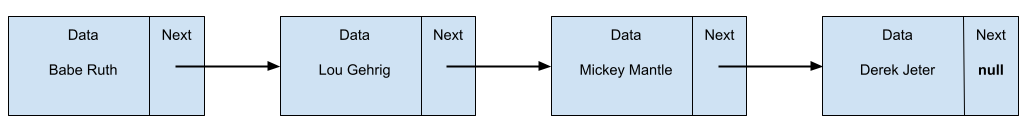
\includegraphics[width=15cm]{linkedList}
    \caption{Example singly linked list of 4 Yankees legends.}
    \label{figure:linkedList}
 \end{figure}

\subsection{Asymptotic Analysis}
Assuming one only has a pointer to the first element in the list, doing any sort of work with the data requires one to start at the beginning and traverse through the list by using the next pointer within each node until the desired operation is complete. For example, as done in Listing \ref{lst:maincpp} within Section \ref{mainProgramListing} on lines 22-26, the only way to dynamically obtain the data for each node was to start at the beginning and iterate through each node by taking advantage of the links. Overall, since linked list operations, such as searching, adding, and removing, all function at a rate of a magnitude of the size of the list, their runtime is classified as $O(n)$.

\subsection{Good Parts of the Implementation of a Singly Linked List}
\subsubsection{Limited Size Restrictions}
As previously mentioned in Section \ref{linkedListDataStructure}, the last node within a linked list has a next of \textbf{null}. This characteristic enables linked lists to have no size restrictions barring memory capacity. As a result, this feature makes linked lists preferred over arrays, which have a fixed length, when the size of the data is frequently changing and has an unkown maximum. For instance, as demonstrated in Listing \ref{lst:maincpp} of Section \ref{mainProgramListing} on lines 13-19, the size of the linked list is only limited by our needs and, if needed, more nodes are able to easily be added to the list with their creation as done on lines 13-15 and linking as shown on lines 18 and 19. On the other hand, if the list was made with an array, the size of the array would have to be provided at the time of creation, and it would not be easy to change the size if additional data have to be added to the array.

\subsubsection{Data Type Flexibility}\label{linkedListDataType}
Linked lists do not have to be restricted to be able to store a specific data type. Instead, with the use of generics (C++ templates), the definition of a node is independent of the data type that the user wants to store within the linked list. This provides flexibilty and reusability for many use cases. As demonstrated in Section \ref{nodeListing} Listing \ref{lst:nodeh}, the definition of a node uses a generic T as the type of data being stored, which prevents any assumptions of the data and ensures compatibility with all data types. However, due to how the C++ linker works and to prevent all the code from being written within a single header file, the allowed types have to be stated on lines 13 and 14 in Listing \ref{lst:nodecpp}. This is a C++ specific issue and is not present in other languages such as Java. Regardless, although they have to be specified for C++, any data type can still be stored within a node and a linked list. A demonstration of the user defining which data type is stored in a node is in Section \ref{mainProgramListing} on lines 13-15 of Listing \ref{lst:maincpp}. Instead of the Node class defining the data type, the user is able to specify the type of data they want to store, which is a string in this situation but can be anything they want.

\section{Stack}
\subsection{The Data Structure}\label{stackDataStructure}
A stack uses a last in, first out (LIFO) approach to storing data. The most common analogy for stacks is a stack of plates. Each plate is placed on top of each other to build the stack when being stored, but the plate on top is always the first to be used. In other words, the most recent plate that was put away is also the first plate that is taken out. As displayed in Figure \ref{figure:stack}, the stack has a variable called top, which points to the first item in the stack. Additionally, as shown by the arrows between each element, linked lists are used in the implementation of stacks. Stacks have 3 primary functions: push, pop, and isEmpty. Push adds a new element to the top of the stack, pop removes the top item from the stack and returns the item, and isEmpty returns whether or not the stack is empty.

\begin{figure}[ht] 
    \centering 
    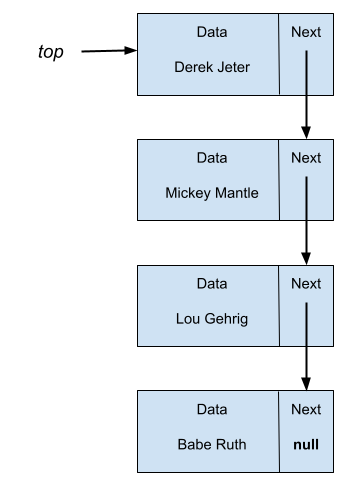
\includegraphics[height=6cm]{stack}
    \caption{Example stack of 4 Yankees legends.}
    \label{figure:stack}
 \end{figure}

\subsection{Asymptotic Analysis}\label{stackAnalysis}
Stacks are incredibly fast when it comes to the implementation of its methods. As demonstrated in Listing \ref{lst:stackcpp} in Section \ref{stackListing}, the push method on lines 14-21 points the new element's next to the current top of the stack (line 17) and updates the top of the stack to point to the new node (line 18). These 2 steps will always run and do not depend on the current size of the stack, which means that the push method runs in $O(1)$ time. The pop method on lines 24-40 is very similar in that it also executes the same few steps regardless of the current size of the stack. These steps are check if the stack is empty for safety (lines 26-29), grab the node from the top of the stack (line 31), update the top pointer to point to the second item in the stack (line 32), update the old top by making it not point to another node (line 36), and return the old top node (line 38). There is no need to traverse the list because the push method made the new node the first element of the list, which is equivalent to the top of the stack. Therefore, just like the push method, the pop method also runs in $O(1)$ time. Lastly, the isEmpty method simply returns the result of the boolean expression on line 45, which also makes it run in $O(1)$ time.

\section{Queue}
\subsection{The Data Structure}\label{queueDataStructure}
A queue uses a first in, first out (FIFO) approach to handling data. One analogy to understand how a queue works is a line to buy movie tickets. The first person that is in line for these tickets is the first to be assisted at the ticket counter. On the other hand, the last person to enter the line will also be the last one to buy their ticket. Similar to stacks, queues are implemented using a singly linked list. As displayed in Figure \ref{figure:queue}, queues have a head variable that points to the first node within the linked list, which equates to the front of the line for the movie tickets. Although not needed to implement a queue, a tail pointer to the last element in the queue may also be provided for efficiency, which is described more in detail in Section \ref{queueAnalysis}. Lastly, queues have 3 primary functions: enqueue, dequeue, and isEmpty. Enqueue adds a new element to the end of the queue, dequeue removes and returns the first element in the queue, and isEmpty checks to see if the queue is empty or not.

\begin{figure}[ht] 
    \centering 
    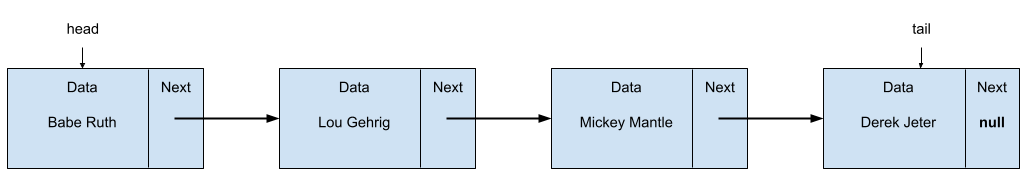
\includegraphics[width=15cm]{queue}
    \caption{Example queue of 4 Yankees legends.}
    \label{figure:queue}
\end{figure}

\subsection{Asymptotic Analysis}\label{queueAnalysis}
Similar to stacks, queues are also very efficient in the implementation of their respective methods. First, the enqueue method has different run times dependent on the implementation of the data structure. If there is no tail pointer, then one would have to start at the head and then traverse through the list and then set the new node to be the next of the last node in the queue. This implementation results in $O(n)$ runtime because it only loops through the list once. The other implementation of a queue with a tail pointer, despite its need for a little extra memory, greatly reduces the runtime of the enqueue method. As shown in Listing~\ref{lst:queuecpp} of Section \ref{queueListing} on lines 23 and 24, the addition of the tail pointer prevents the need to traverse through the list and, instead, immediately adds the new node to the queue. Since there are now a fixed number of steps regardless of the size of the queue, the new runtime of the enqueue method is $O(1)$. Next, in addition to the update to the tail pointer if the queue is empty after dequeuing an element on lines 39-42 of Listing \ref{lst:queuecpp} of Section \ref{queueListing}, the dequeue method is identical to the pop method from the Stack class (see Section \ref{stackAnalysis}), which classifies it as constant time $O(1)$. Lastly, the isEmpty method also runs in $O(1)$ time because it only executes and returns the result of the boolean expression.

\section{Good Parts of the Implementation of Stacks and Queues}
\subsection{Compatibility with the Node Class}\label{nodeCompatibility}
As mentioned in Sections \ref{stackDataStructure} and \ref{queueDataStructure}, stacks and queues are both implemented using singly linked lists. Therefore, they both have to be able to utilize the Node class for singly linked lists. On line 9 of Listing \ref{lst:stackh} in Section \ref{stackListing} as well as lines 9 and 12 of Listing \ref{lst:queueh} in Section \ref{queueListing}, each of the variables are declared using the template, which defines the data type that the nodes are allowed to use within the stack and queue. The definition of the data type to be used by the stack or queue can be found on lines 32 and 62 of Listing \ref{lst:maincpp} of Section \ref{mainProgramListing} at the time of creation of the data structures. This data type is a strict definition for what is being used by the data structure, which means that only that data type can be used. Lines 88 and 89 of Listing \ref{lst:maincpp} in Section \ref{mainProgramListing} does not compile because a node with string data cannot be used within a queue for characters, which is why the code is commented out.

\subsection{Error Safety}
In addition the the type safety of the templates as described in Section \ref{nodeCompatibility}, the Stack and Queue classes also have an error measure to prevent users from breaking the program by doing something that is not allowed. The error safety occurs if the user tries to pop from an empty stack or dequeue from an empty queue. As displayed on lines 26-29 of Listing \ref{lst:stackcpp} in Section \ref{stackListing} as well as lines 32-35 of Listing \ref{lst:queuecpp} in Section \ref{queueListing}, both the pop and dequeue functions check if the respective data structure is empty and throws an error if it is. This is really important as, without the check, there would be a runtime error that crashes the program from attempting to work with a null pointer. This check impacts how the data structures are used. For instance, in the test program for the queue in Listing \ref{lst:maincpp} of Section \ref{mainProgramListing}, lines 80-85 use a try-catch block to make sure the programmed error is thrown when attempting to dequeue from the empty queue.

\section{Main Program}
\subsection{Program Overview}\label{mainOverview}
The objective of the main program was to print out all the palindromes, ignoring whitespace and capitalization, within a file. More specifically, after normalizing a string for whitespace and capitalization, each character of the string should be both pushed onto a stack and enqueued on a queue. The stack will hold the characters in reverse order and the queue will hold each character in the order as they are in the string. Thus, checking to see if the string is a palindrome requires one to just pop the first character from the stack and dequeue the first character in the queue. If there is ever a time where the characters are different, then the string is not a palindrome. On the other hand, if every comparison is successful, then the string is a palindrome.

\subsection{Asymptotic Analysis}
The main program contains 2 main components: the file reading and the isPalindrome function. First, the file reading function, as shown in Listing \ref{lst:fileutilcpp} in Section \ref{mainProgramListing}, consists of 2 loops that each read through the entirety of the file. The first loop (lines 20-24) is used to determine the number of items in the file so the array can be properly made, and the second loop (lines 39-43) saves the contents of the file into the array. Since each loop iterates for the number of elements in the data and has a fixed number of steps in each iteration, the runtime of the file reading is $O(2n)$, which simplifies to $O(n)$. Next, the isPalindrome function on lines 93-138 of Listing \ref{lst:maincpp} in Section \ref{mainProgramListing} has a very similar situation for the runtime complexity. The function begins by iterating through each character of the string and pushing and enqueuing the character to the stack and queue (lines 99-115). Since these functions both run in $O(1)$ time, we can say there are a fixed number of steps for each iteration of the loop. The other loop (lines 117-134) pops and dequeues the stack and queue and performs the comparison described in Section \ref{mainOverview}. Similar to the first loop, since pop and dequeue have runtimes of $O(1)$, there are a fixed number of steps within each iteration of the second loop as well. Therefore, the runtime complexity of isPalindrome, just like the file reading, has an overall runtime complexity of $O(2n)$, which simplifies to $O(n)$.

\subsection{Good Parts of the Program's Implementation}
\subsubsection{The StringArr Struct}
As the data has to be read into an array, the program needs access to it outside of the file reading function. Thus, the array needs to be declared on the heap, as shown on line 28 of Listing \ref{lst:fileutilcpp} of Section \ref{mainProgramListing}, so the array will not be destroyed at the end of the function and the pointer to the array can be used outside the scope of the function. The number of elements of an array in C++ is typically the size of the overall array divided by the size of an individual element. However, since the array was declared on the heap, the length of the array is unkown because we only have the pointer to the first element, which is always 8 bytes. Therefore, as shown on lines 5-9 of Listing \ref{lst:utilh} in Section \ref{mainProgramListing}, the definition of the StringArr struct helps with this issue as it stores the pointer to the array as well as the number of elements in the array. This is crucial for the program as it can now loop through each element of the array, which is demonstrated on line 168 of Listing~\ref{lst:maincpp} in Section \ref{mainProgramListing}.

\section{Appendix}
\lstset{numbers=left, numberstyle=\tiny, stepnumber=1, numbersep=5pt}

% Colors and lstset for syntax highlighting from https://www.overleaf.com/latex/examples/syntax-highlighting-in-latex-with-the-listings-package/jxnppmxxvsvk
\definecolor{mygreen}{rgb}{0,0.6,0}
\definecolor{mygray}{rgb}{0.5,0.5,0.5}
\definecolor{mymauve}{rgb}{0.58,0,0.82}
\lstset{
  backgroundcolor=\color{white},   % choose the background color
  basicstyle=\footnotesize,        % size of fonts used for the code
  breaklines=true,                 % automatic line breaking only at whitespace
  captionpos=b,                    % sets the caption-position to bottom
  commentstyle=\color{mygreen},    % comment style
  escapeinside={\%*}{*)},          % if you want to add LaTeX within your code
  keywordstyle=\color{blue},       % keyword style
  stringstyle=\color{mymauve},     % string literal style
}

\subsection{Singly Linked List}\label{nodeListing}
\lstinputlisting[caption=node.cpp, label=lst:nodecpp, language=C++]{./../node.cpp}
\lstinputlisting[caption=node.h, label=lst:nodeh, language=C++]{./../node.h}

\subsection{Stack}\label{stackListing}
\lstinputlisting[caption=stack.cpp, label=lst:stackcpp, language=C++]{./../stack.cpp}
\lstinputlisting[caption=stack.h, label=lst:stackh, language=C++]{./../stack.h}

\subsection{Queue}\label{queueListing}
\lstinputlisting[caption=queue.cpp, label=lst:queuecpp, language=C++]{./../queue.cpp}
\lstinputlisting[caption=queue.h, label=lst:queueh, language=C++]{./../queue.h}

\subsection{Main Program}\label{mainProgramListing}
\lstinputlisting[caption=main.cpp, label=lst:maincpp, language=C++]{./../main.cpp}
\lstinputlisting[caption=fileUtil.cpp, label=lst:fileutilcpp, language=C++]{./../fileUtil.cpp}
\lstinputlisting[caption=util.h, label=lst:utilh, language=C++]{./../util.h}

\end{document}